% Currently this document is written in English
% !TeX encoding = UTF-8
% !TeX spellcheck = en_US
% !TeX program = pdflatex
% !BIB program = biber

%Ensure that all odl school LaTeX habits are remarked
\RequirePackage[l2tabu, orthodox]{nag}

%German: remove "english"
\documentclass[english,utf8,biblatex,noeditorial]{lni-tex/lni}
% Nice tables using \toprule, \midrule, \bottomrule
\usepackage{booktabs}
\usepackage{multirow}
% custom enums (more compact)
\usepackage{enumitem}
\setlist{noitemsep,topsep=0pt,parsep=0pt,partopsep=0pt}
% subfigures and subcaptions
\usepackage{subcaption}

%% Begin: Drawings
% use standalone and tikz for high-fid. drawings

% standalone package and config
\usepackage{standalone} % For pre-compiled pictures
\standaloneconfig{mode=buildnew} % only build image if source file is newer

% tikz package and config
\usepackage{tikz} % For Tikz pictures
\usetikzlibrary{
  positioning,
  fit,
  arrows,
  calc,
  backgrounds
}

% pgfplots
\usepackage{pgfplots}
\pgfplotsset{compat=1.16} % set pgfplots compatibility to version 1.16

\graphicspath{{pictures/tikz/}{pictures/png/}}
%% End: Drawings

%% Begin: Biblatex

%for easy quotations: \enquote{text}, also required by biblatex
\usepackage{csquotes}
% biblatex is included with LNI-class option: `biblatex`, only set bibliography-file:
\bibliography{paper}

% Clear fields we do not need
\iffalse
\AtEveryBibitem{%
  \ifentrytype{article}{%
  }{%
    \clearfield{doi}%
    \clearfield{issn}%
    \clearfield{url}%
    \clearfield{urldate}%
  }%
  \ifentrytype{inproceedings}{%
  }{%
    \clearfield{doi}%
    \clearfield{issn}%
    \clearfield{url}%
    \clearfield{urldate}%
  }%
}
\fi
%% End: Biblatex

%% Begin: lstlistings

% configuration of lstlisting
\lstset{%
	xleftmargin=0.5cm, % expected by LNI
  captionpos=b,      % expected by LNI
  fontadjust=true,
  columns=[c]fixed,
  keepspaces=true,
  tabsize=2,
  basicstyle=\renewcommand{\baselinestretch}{0.95}\ttfamily,
  commentstyle=\itshape,
  keywordstyle=\bfseries,
  mathescape=true,
  escapechar=§,
}

% macro for inline code
\newcommand{\code}[1]{\lstinline[flexiblecolumns=true,basicstyle=\renewcommand{\baselinestretch}{0.95}\ttfamily]{#1}}

%% End: lstlistings

%% Begin: Acronyms
\usepackage[acronym]{glossaries}
\glsdisablehyper

% define acronyms here:
\newacronym{jvm}{JVM}{Java Virtual Machine}
\newacronym{paas}{PaaS}{Platform as a Service}

% define special names here (we do not create a glossary, so no descriptions are required)
\newglossaryentry{kubernetes}{name={Kubernetes},plural={Kubernetes},description={}}
%% End: Acronyms


%% Begin: Macros
% \newcommand{\reactdb}[1]{\textsc{ReactDB}}
\lniabbrv{\etc}{etc.}
%% End: Macros


%% correct bad hyphenation here
\hyphenation{net-works semi-conduc-tor}


% Start of page count 
% ----------------------- filled out by publisher/editor
%\startpage{1}
%\editor{Sebastian Schmidl}
%\booktitle{Technical Report}
%\year{2019}
% -----------------------

\author[Sebastian Schmidl]{%
  Sebastian Schmidl%
  \footnote{%
    Hasso Plattner Institut, University of Potsdam, Prof.-Dr.-Helmert-Str. 2-3, 14482 Potsdam, %
    \email{sebastian.schmidl@student.hpi.de}%
  }%
}
\title[Self-Healing Microservices with Kubernetes]{Self-Healing Microservices with Kubernetes}
\subtitle{Self-Adaptation in Micro-Service Architectures with Kubernetes Seminar -- Summer Term 2019}

\begin{document}
\maketitle

% Set to number of authors!
% Authors use each one footnote counter, set this to align the remaining ones.
% E.g. 2 authors --> set to 2, next footnote will be 3
\setcounter{footnote}{1}

\begin{abstract}
  Abstract goes here.
\end{abstract}

\begin{keywords}
Self-Adaptive Systems \and Self-Healing \and Microservices \and Cloud Computing \and Kubernetes \and Decentralized \and Distributed \and Orchestration
\end{keywords}

% Contents
% --------
% !TeX root = paper.tex
% !TeX encoding = UTF-8
% !TeX spellcheck = en_US

% Outline of this paper

\glsresetall
% !TeX root = ../paper.tex
% !TeX encoding = UTF-8
% !TeX spellcheck = en_US

\section{Introduction}\label{sec:introduction}
  Introduce the topic.
  


% !TeX root = ../paper.tex
% !TeX encoding = UTF-8
% !TeX spellcheck = en_US

\section{Self-Healing}\label{sec:self-healing}
  Self-healing is an integral part of self-adaptive systems and the focus of this paper.
  It combines properties of
  (i) fault-tolerant systems, which handle transient failures and mask permanent ones to ensure system availability,
  (ii) self-stabilizing systems, which are non-fault masking and converge to the legal state in a finite amount of time, and 
  (iii) survivable systems, which maintain essential services and recover non-essential ones after intrusions have been dealt with~\cite{PsaierSurvey}.
  A widely-used definition for self-healing systems is from \citeauthor{Ghosh}~\cite{Ghosh}:

  \begin{quote}
    The key focus [...] is that a self-healing system should recover from the abnormal (or \enquote{unhealthy}) state and return to the normative (\enquote{healthy}) state, and function as it was prior to disruption.
  \end{quote}

  This definition is very broad, but one can argue that the key aspect of self-healing systems are recovery oriented functionalities that bring the system back to the healthy state, which neither sole fault-tolerant systems nor sole survivable systems encompass~\cite{PsaierSurvey}.

  Like in an autonomous system, the main component in a self-healing system is the self-healing manager.
  It runs a control loop with three stages that is a reduced version of the autonomic control loop, also referred to as MAPE-K loop~\cite{ibm_autonomic}.
  The self-healing loop consists of the following three main stages~\cite{PsaierSurvey}:

  \begin{description}
    \item[Detect] The self-healing manager filters the status information about the running system and reports suspicious events and detected degradations.
    \item[Diagnose] The diagnosis stage performs root cause analysis on the received reports from the previous stage and calculates a recovery strategy.
    \item[Recover] In the recovery phase the manager applies the strategies to the system while he avoids any unpredictable side effects.
  \end{description}

  These three stages reflect the definition of self-healing.
  \Cref{fig:self-healing-loop} shows the mapping of those stages to the MAPE-K control loop.
  There are two different ways, how a software system can be equipped with the above mentioned self-healing capabilities:

  \begin{figure}
    \centering
    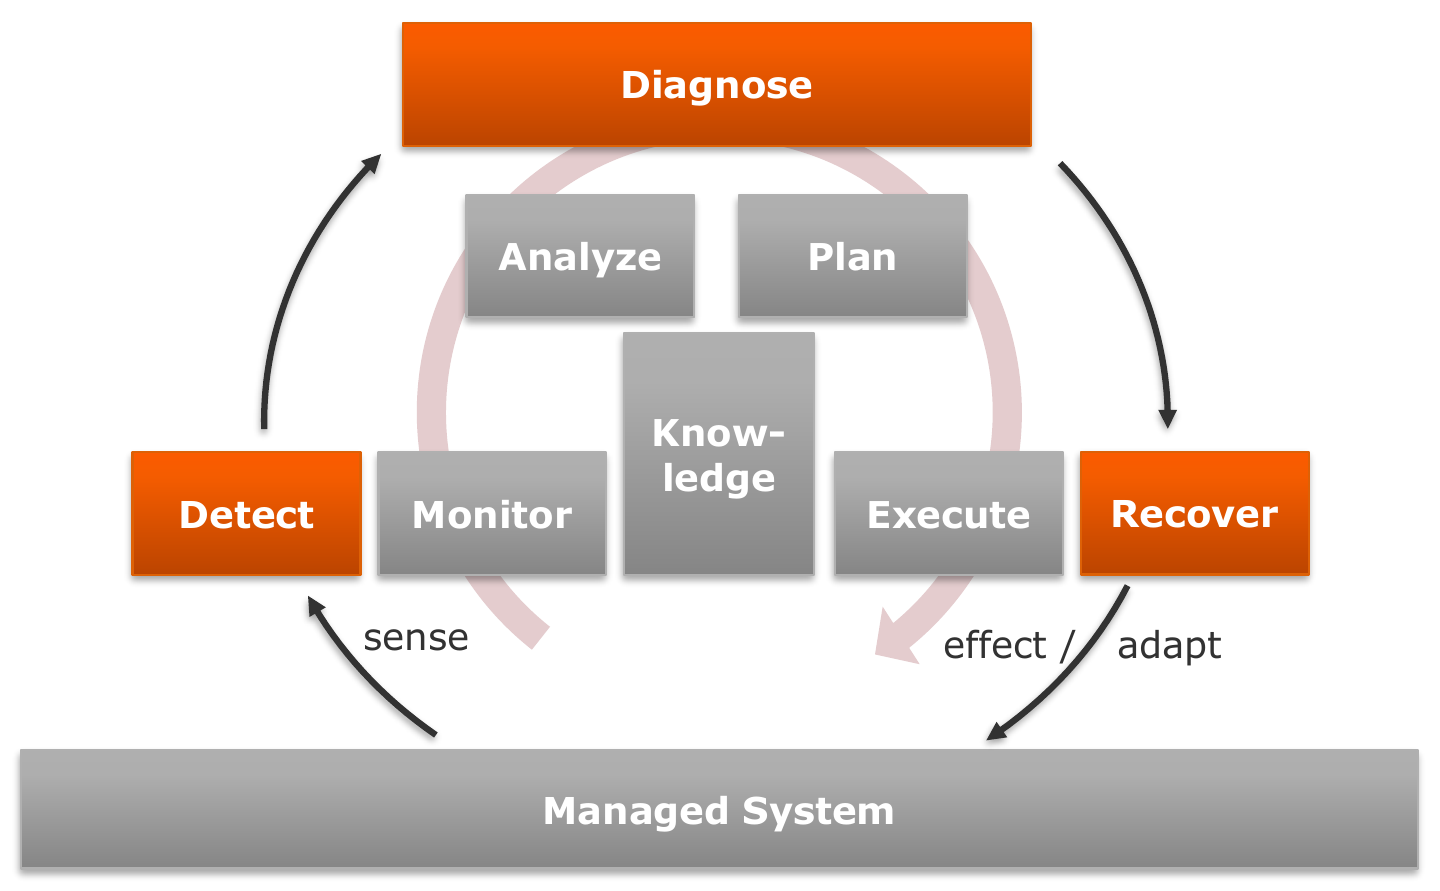
\includegraphics[width=\linewidth]{reduced-control-loop}
    \caption{Condensed autonomic control loop as the self-healing loop}
    \label{fig:self-healing-loop}
  \end{figure}

  The first approach is a software application with built-in self-healing logic.
  This means that the self-healing manager is within the application code and is able to access internal state and mechanisms.
  This can be an advantage as the application is a white box and the self-healing logic can use detailed status information and even domain knowledge for detection, analysis and recovery.
  At the other hand, this also means that the healing logic is tied to the application increasing coupling and violating the separation of concerns principle.
  If the application starves the self-healing manager may starve as well.

  The second approach is an external self-healing manager provided as an infrastructural component or as third-party service.
  The self-healing logic runs in isolation from the application code and can therefore treat the application only as a black box and has to use external metrics to judge the application's health.
  It's the current state of the art for monitoring, health management and scaling logic~\cite{ToffettiMicroservices}.
  The external management logic has to be itself resilient, fault-tolerant, and scalable for being able to heal the application.
  Using third party services or services provided by the infrastructure provider could lead to vendor lock-in.
  There are also open-source alternatives that include self-healing capabilities and can be used as middleware between cloud infrastructure and the application, such as \gls{kubernetes} or Mesosphere.

\subsection{Architecture-based self-healing}
  In the past most self-healing capabilities were included in the application code itself.
  This has the downside that the self-healing adaption engines and rules are tightly coupled to the application code and can't be reused.
  Researchers have therefore developed ways to generalize self-healing mechanisms.
  One approach are architecture-based self-healing systems, in which external self-healing managers perform repairs on the level of software components and connectors of the monitored systems~\cite{DashofyArchitecture}.
  The assumption of those approaches is that the component boundaries are the most loosely coupled points in the software system and can be reconfigured to allow changes in the architecture during runtime.

  \citeauthor{DashofyArchitecture} present the infrastructure to develop and run an architecture-based self-healing system that focuses on event-based software architectures in~\cite{DashofyArchitecture}.
  They chose event-based architectures, because all included components can only communicate via events and show a significant degree of autonomy.
  This reduces coupling of the components and makes changes from the outside to the system possible.

\subsection{Self-healing microservices}
  Microservice architectures take isolation of software components to the next level and improve the autonomy of the components (services).
  This makes applying repairs from the outside of the application easier, because services are decoupled, autonomous, and scalable and service boundaries are well-defined.
  External self-healing managers can monitor the microservices of the application and apply repairs to the failing or misbehaving ones by replacing the service with another one and rerouting the messages to the new instance.
  This is where the self-healing capabilities of the aforementioned cloud tools (refer to \cref{sec:introduction}) and \gls{kubernetes} can be used.

  In contrast to external self-healing managers, \citeauthor{ToffettiMicroservices} propose a self-healing system with the self-healing logic built into a microservice application.
  They leverage standard methods from distributed systems (\ie consensus algorithms) to assign self-management (includes self-healing) functionality to some nodes of the distributed application.
  The selected nodes form a hierarchy and perform different parts of the self-management logic.
  This means that the self-management logic is distributed in the cluster to overcome the connectedness to the application code~\cite{ToffettiMicroservices}.

\subsection{Self-healing challenges in cloud environments}
  While systems and software components can fail in various ways and research has come up with general failure classifications and resolutions~\cite[Tab.~1]{PsaierSurvey} for any software systems, failures in cloud environments can be reduced to one failure class: a node or component is detected unreachable.
  Although an unreachable node can have different root causes on the infrastructure level, the impact on the system is the same and we have no control about the infrastructure in a cloud deployment.
  This means that we have to find other ways besides repairing the infrastructure to heal from those failures.
  Node failures can be detected via heartbeat messages or latency metrics and a common recovery strategy used is the restart of the software that was running on the node on another node.

  \begin{quote}
    In the pre-cloud days, this would have been pretty manual, some poor sap of an engineer would have to nurse a bare metal or VM back to health.
    Now, with cloud-based abstractions, individual compute units are much more expendable.
    We can just take them down and replace them with new ones.
  \end{quote}

  \begin{itemize}
    \item self-healing manager must be resilient itself
    \item Reactive Manifesto~\cite{reactivemanifesto} asks for more resilient and responsive systems.
    The resilience is achieved by replication, containment, isolation, and delegation.
    Recovery should be handled by an external component.
    This could be a self-healing component.
    \item \cite{StackCloud}
      \begin{itemize}
        \item hierarchical approach
        \item layered master-slave architecture to provide flexibility and high availability
        \item targets decentralized cloud architectures
      \end{itemize}
    \item \cite{gru}
      \begin{itemize}
      \item similar to this approach, but they have developed their own container orchestration tool, called Gru, instead of using \gls{kubernetes}
      \item also targets microservice architectures deployed in containers
    \end{itemize}
  \end{itemize}

\section[Kubernetes]{\gls{kubernetes}}\label{sec:kubernetes}
  % https://kubernetes.io/docs/concepts/overview/what-is-kubernetes/
  \Gls{kubernetes} is an open-source platform for automating and managing distributed software in the cloud.
  It heavily relies on container technology and supports the declarative configuration of the managed containers.
  \Gls{kubernetes} was developed by Google and is open-source software since 2014~\cite{kubernetes}.

  % https://kubernetes.io/docs/concepts/overview/components/
  \Gls{kubernetes} is build on top of existing \gls{paas} solutions and consists of a master-slave architecture, which is depicted in \cref{fig:kubernetes-architecture}, forming a cluster.
  Slave nodes, \gls{kubernetes} calls them only \enquote{nodes}, are responsible for executing and maintaining the actual application via an underlying container runtime.
  Most of the time Docker~\cite{docker} is used.
  The nodes also run \gls{kubernetes} components that manage cluster networking (\texttt{kube-proxy}) and interact with the container runtime and the master to monitor and manage the pods of the local node (\texttt{kubelet}).
  % https://kubernetes.io/docs/concepts/workloads/pods/pod-overview/
  Pods are the smallest deployment unit in \gls{kubernetes} and consist of the application container (or multiple), connected resources, such as storages or network addresses, and the configuration options.
  The container runtime, \texttt{kube-proxy} and \texttt{kubelet} form the \gls{kubernetes} runtime environment~\cite{kubernetes}.

  \begin{figure}
    \centering
    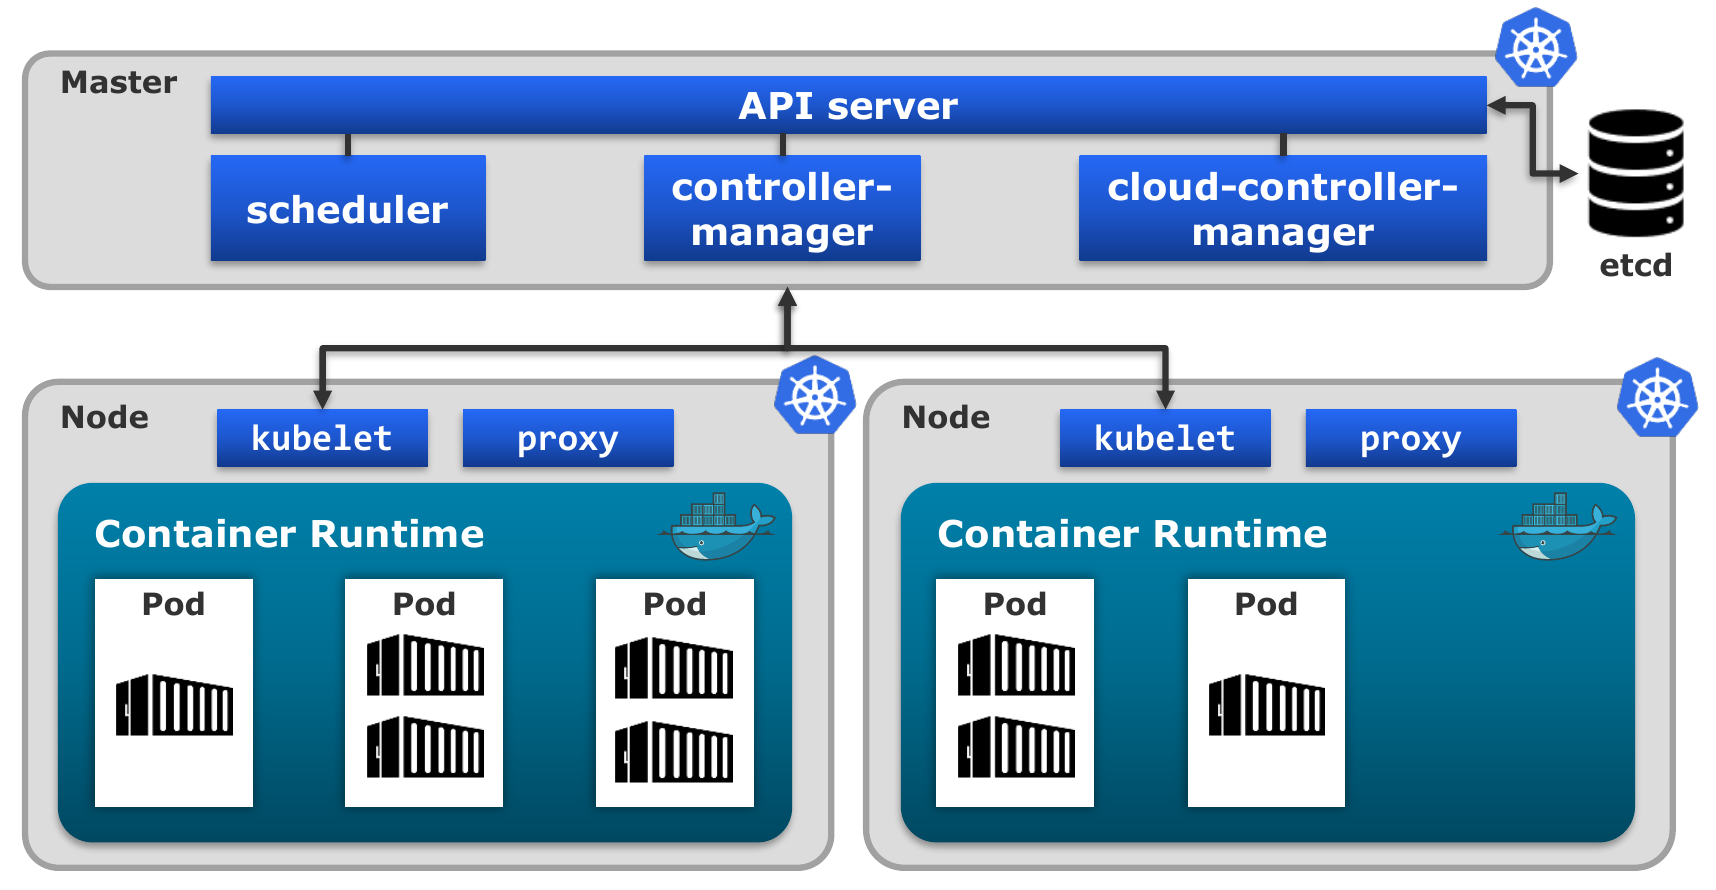
\includegraphics[width=\linewidth]{k8s-architecture}
    \caption{\Gls{kubernetes} architecture}
    \label{fig:kubernetes-architecture}
  \end{figure}

  The \gls{kubernetes} master components provide the cluster's control plane.
  As shown in the upper third of \cref{fig:kubernetes-architecture}, they typically run only on one node, which does not run application pods.
  However, the components can be executed on any node in the cluster.
  The master components include
  (i) the \texttt{kube-apiserver} that exposes the control options to the user and other software,
  (ii) an \texttt{etcd}~\cite{etcd} instance as store for all cluster data,
  (iii) the \texttt{kube-scheduler}, which schedules newly created pods to the nodes in the cluster,
  (iv) the \texttt{kube-controller-manager}, which runs node and pod controllers, and
  (v) the \texttt{cloud-controller-manager} to interact with the underlying cloud providers~\cite{kubernetes}.

  % https://kubernetes.io/docs/concepts/overview/working-with-objects/kubernetes-objects/
  For the declarative configuration and management of the application, \gls{kubernetes} employs the \gls{kubernetes} object model.
  All entities of the \gls{kubernetes} runtime are represented as description objects.
  The entirety of those objects represents the cluster state.
  Each object consists of three parts:
  (i) the object's metadata, such as name, version or labels,
  (ii) the object \texttt{spec}, which describes the desired state for the object and is provided by the user, and
  (iii) the object \texttt{status}, which describes the actual state of the object.
  Users of \gls{kubernetes} therefore only provide the object's metadata and \texttt{spec} to declare the desired deployment of their containerized applications on nodes and policies around how the application should behave.
  \Gls{kubernetes} will constantly update the \texttt{state} of the objects according to the observed cluster state and take corrective actions in the cluster to ensure that the cluster state matches the desired one declared in the objects' \texttt{spec}~\cite{kubernetes}.

  % https://kubernetes.io/docs/concepts/overview/working-with-objects/labels/https://kubernetes.io/docs/concepts/overview/working-with-objects/labels/
  % should I describe labels as well?


% !TeX root = ../paper.tex
% !TeX encoding = UTF-8
% !TeX spellcheck = en_US

\section{\Gls{kubernetes}' self-healing capabilities}\label{sec:self-healing-kubernetes}
  In this section we will go through the self-healing capabilities available in \gls{kubernetes}.
  We will start with a short overview how \gls{kubernetes} approaches self-healing and what failure types exist in \cref{sec:self-healing-kubernetes:overview}.
  We then explain, how \gls{kubernetes} implements the three properties of self-healing systems: fault-tolerant in \cref{sec:self-healing-kubernetes:fault-tolerant}, self-stabilizing in \cref{sec:self-healing-kubernetes:self-stabilizing} and survivable in \cref{sec:self-healing-kubernetes:survivable}.

\subsection{Overview}\label{sec:self-healing-kubernetes:overview}
  \gls{kubernetes}' self-healing capabilities are spread across various components and functionalities, but in essence they also perform the three-staged self-healing loop introduced in \cref{sec:self-healing}.
  \gls{kubernetes}' approach to self-healing is comparable to architecture-based self-healing~\cite{ToffettiMicroservices,DashofyArchitecture}.
  Its declarative object configuration model resembles the concept of a desired and actual runtime architecture of the managed application.
  The user of \gls{kubernetes}
  %, which can also be another software program as the \gls{kubernetes} API is machine-readable,
  can define the desired system architecture as the \texttt{spec} part of the deployment configuration.
  % \citeauthor{ToffettiMicroservices} call this the \textit{instance graph}~\cite{ToffettiMicroservices}.
  It is stored by the master components in \texttt{etcd}.
  \Gls{kubernetes} then internally creates the \texttt{state} part of the objects in \texttt{etcd} by monitoring the actual nodes and pods in the cluster.
  This will detect failures in the cluster.
  The \texttt{state}s represent the current architecture of the running components and are continuously updated.
  Based on those two representations corrective measures can then be calculated during the diagnosing stage.
  \Gls{kubernetes} applies them to the cluster fully automatically to recover from failures.
  The actual state of the system thereby converges to the desired one.

  There are two levels of disruptions that can occur in a \gls{kubernetes} deployment: Container failure and pod disruptions.
  % https://kubernetes.io/docs/concepts/workloads/pods/pod-lifecycle/\#restart-policy
  Containers are runtime artifacts defined by users and can therefore fail or crash during execution.
  Those container failures are captured by the restart policy of their pod objects.
  When the restart policy is set to \textit{Always} or \textit{OnFailure}, failing containers are automatically restarted by the local \texttt{kubelet} component with an exponential back-off strategy.
  In this special case the self-healing loop is performed by the local \texttt{kubelet} component on each node.

  In contrast to containers, pods do not disappear until someone (the user or a \gls{kubernetes} component) destroys them or there is an unavoidable system error.
  \Gls{kubernetes} considers the following involuntary disruptions for pods~\cite{kubernetes}:

  \begin{itemize}
    \item a hardware failure of the physical machine backing the node
    \item cloud provider or hypervisor failure makes VM disappear
    \item administrator deletes VM by mistake
    \item a kernel panic of the operating system
    \item a cluster network partition removes the node from the cluster
  \end{itemize}

  % https://kubernetes.io/docs/concepts/workloads/pods/pod-lifecycle/\#pod-lifetime
  All those cases deal with failures of nodes or their communication.
  Therefore, \gls{kubernetes} employs \textit{node-controllers} run by the \textit{controller-manager} in the control plane (see \cref{fig:kubernetes-architecture}) to monitor nodes.
  They detect node failures through a heartbeat-based failure detector and set the phase of all pods that where running on the failed node to \textit{Failed}.
  This summarizes those failures into one category and propagates it to all the pods running on the node.
  This means the self-healing logic in \gls{kubernetes} only has to consider pod failures,
  thus we will only talk about healing from pod failures for the remainder of this section.

  The following three sections explain how \gls{kubernetes} implements the three properties of self-healing systems introduced in \cref{sec:self-healing} to heal from pod failures.
  % with services, \glspl{pod controller}, \glspl{priority class}, and \glspl{pdb}.

\subsection{Fault-tolerant}\label{sec:self-healing-kubernetes:fault-tolerant}
  \Gls{kubernetes} uses pods and containers to isolate different parts of the managed application from one another.
  This fits well for microservice architectures and creates failure domains.
  \Gls{kubernetes} can only provide fault-tolerance if the managed application makes use of pod replication and \glspl{service}.

  Pod replication means that for each microservice type, we let \gls{kubernetes} create multiple pods with the same configuration and containers.
  This means that we run multiple microservice instances at the same time.
  The \texttt{kube scheduler} automatically spreads those replicas across the available nodes to increase the failure tolerance{\url{https://kubernetes.io/docs/concepts/configuration/assign-pod-node/}}.
  This allows other replicas to take over the workload if one replica fails through an involuntary disruption.

  To allow external services to communicate with our replicas, we must be able to reroute the traffic from failing pods to the remaining ones.
  This is done by specifying a \gls{service}, which exposes the set of replicated pods to the cluster internal and external network.
  It performs the load balancing and rerouting of the network traffic to the changing pod instances.
  This decouples the service access from the actual placement and deployment of the pods.

\subsection{Self-stabilizing}\label{sec:self-healing-kubernetes:self-stabilizing}
  Pods can be created manually, but this means the user has to take care of recovering failed pods.
  A better solution is to use \glspl{pod controller}.
  They take pod description objects and manage their pods automatically.
  \Glspl{pod controller} execute the Detect -- Analyze -- Recover loop and run in the \texttt{kube-controller-manager} as a master component.
  \Glspl{pod controller} monitor the health of their managed pods via heartbeats and user-defined liveness probes\footnote{\url{https://kubernetes.io/docs/tasks/configure-pod-container/configure-liveness-readiness-probes/}}.
  Based on this monitoring the \texttt{state} part of the descriptor object is continuously updated to reflect the actual system state.
  Based on the desired state, the current system state, and the policies in the object, the \gls{pod controller} derives corrective actions to transition the system from the current into the desired state.
  In the case of a failed pod, the controller would for example instruct the deletion of the failed pod and the creation of a new one with the same properties.
  The \gls{pod controller} not only contains the self-healing logic for pods but also handles pod replication, rollout, and transparent pod placement on the available nodes.
  Using \glspl{pod controller}, \gls{kubernetes} is able to recover failed pods and to eventually let the actual state converge to the desired one.
  This means applications managed by \gls{kubernetes} can be self-stabilizing.

  There are four different types of pod payloads, which are unique to their failure handling:
  Stateless services, stateful services, daemons, and jobs.
  This is reflected in \gls{kubernetes} by different controller types.
  The next four sections cover the different aspects we have to consider for the failure handling of the application types.

  \subsubsection{Self-healing of stateless services}
    Stateless services as payloads for \gls{kubernetes} pods are easy to manage, because they can be destroyed and recreated on all nodes without any special resource dependencies.
    A stateless service can be defined via a \texttt{Deployment} or a \texttt{ReplicaSet}.
    In the case of a pod failure, those \glspl{pod controller} instruct the deletion of the failed pod and the creation of a new one according to the supplied \texttt{spec}.
    The placement of the pods on the nodes is transparent and done by the \texttt{kube-scheduler}.
    The controllers always try to match the desired number of replicas.

  \subsubsection{Self-healing of stateful services}
    Stateful services can be defined via the \texttt{StatefulSet} deployment configuration.
    Pods managed by this type of \gls{pod controller} have a unique identity including their name, network ID and configuration.
    They can be connected to \texttt{PersistentVolumes}, which are provided by the underlying infrastructure, such as a \gls{paas} solution.
    \texttt{PersistentVolumes} are used as persistent storage for pods and once connected to a pod, they are also tied to the pods identity.
    If a pod fails, the controller reschedules it, potentially on another node, with the same identity.
    Therefore, the pod will reuse the assigned \texttt{PersistentVolumes} and network IDs.
    Routing of network traffic must be taken care of by creating a headless \gls{service}\footnote{\url{https://kubernetes.io/docs/concepts/services-networking/service/\#headless-services}}.
    Stateful services using \texttt{PersistentVolumes} rely on the availability and fault-tolerance of the volumes provided by the underlying infrastructure.

  \subsubsection{Self-healing of daemons}
    Daemons are application components that should run once on all or selected nodes of the cluster, such as cluster storage, node monitoring, or a log collection component.
    Daemons can be defined via a \texttt{DaemonSet} deployment configuration.
    They ensure that a copy of the daemon runs on all the selected nodes.
    If a node with a daemon fails, no action is taken, as the desired state is still met, just with a reduced number of nodes.
    If a new node is added back to the cluster, the \texttt{DaemonSet} takes care of scheduling the creation of a new copy of the daemon on the newly added node.
    Recovering failed nodes must be done manually.

  \subsubsection{Self-healing of jobs}
    Jobs only run once.
    They can be defined using the \texttt{Job} deployment configuration.
    The job \gls{pod controller} ensures that the job is run to completion.
    This means if the job consists of one pod, this pod must terminate successfully, otherwise it will be restarted.
    Jobs can be started with parallel pods.
    In this case, the use can either specify a number of completions that must succeed or the controller waits for the first pod to successfully terminate.
    If those conditions are not yet met, the controller will recover failed pods.

\subsection{Survivable}\label{sec:self-healing-kubernetes:survivable}
  Survivable systems maintain the essential services of the managed application in the case of failure and resource pressure, while non-essential services may experience disruptions and are recovered after the failure has been dealt with.
  \Gls{kubernetes} provides two ways for the user to influence the pod scheduling algorithm: \glspl{priority class} and \glspl{pdb}.
  They can be used to compile a set of policies that help the scheduler to decide, which pods are essential and how many disruptions a set of replicated pods can handle.

  \Glspl{priority class} map to integer values, where a higher value indicates higher priority, and the user can assign them to the pods.
  Pod priority will affect the scheduling order of the pods.
  Higher priority pods will be scheduled first.
  In addition, under resource pressure higher priority pods in the scheduler queue will lead to lower priority pods being evicted by the scheduler.
  This is called preemption.
  If the user assigns high priority \glspl{priority class} to the essential services, the scheduler will do its best to recreate all instances of the essential services if they fail.
  It will even evict lower priority pods to make room for the essential services\footnote{\url{https://kubernetes.io/docs/concepts/configuration/pod-priority-preemption/}}.

  To prevent the scheduler to evict all instances of a lower priority service, the user can specify \glspl{pdb}.
  They limit the number of replicated pods that are down due to voluntary disruptions, such as draining or preemption.
  Unfortunately, the scheduler only considers \glspl{pdb} on best effort basis during preemption, which limits the applicability of \glspl{pdb} for self-healing\footnote{\url{https://kubernetes.io/docs/concepts/workloads/pods/disruptions/\#how-disruption-budgets-work}}.


% !TeX root = ../paper.tex
% !TeX encoding = UTF-8
% !TeX spellcheck = en_US

\section{Discussion}\label{sec:discussion}
  \begin{enumerate}
    \item requires containerized microservice application
    \item code must support scaling and dynamic communication
    \item provider of \texttt{PersistentVolumes} must ensure their availability and fault-tolerance
    \item to deal with a node failure, remaining nodes must have enough spare capacity to host the failed pods
    \item with replication factor 1, there are down times during re-creation of the pod on another node
    \item limitations
    \begin{itemize}
      \item \textbf{external management logic has to be themselves resilient, fault-tolerant, and scalable}
      \item \gls{kubernetes} default only one master $\rightarrow$ HA setup across availability zones
      \item quite a lot of configuration work, not automation yet (WIP)
      \item only one master will be active (the other two will be passive), full state replication via etcd
      \item fail-over will be handled by load balancer component
      \item \textbf{only external view on the system}
      \item \textbf{\gls{kubernetes} does not automatically repair or restart failing nodes}
      \item --> automatic node repairs on GCE: \url{https://cloud.google.com/kubernetes-engine/docs/how-to/node-auto-repair}
      \item components external to \gls{kubernetes} are not included in self-healing logic (such as external storage or load balancers of cloud provider)
    \end{itemize}
    \item benefits
    \begin{itemize}
      \item healing from pod / container failures and node failures out-of-the-box
      \item declarative definition of system state
      \item rich API to retrieve current system state
    \end{itemize}
    \item interesting facts and insights
  \end{enumerate}

%% !TeX root = ../paper.tex
% !TeX encoding = UTF-8
% !TeX spellcheck = en_US
 
\section{Related Work}\label{sec:related-work}
  \begin{itemize}
    \item \textbf{Is this chapter needed?} I could put a quick rundown of the approaches (\cite{ToffettiMicroservices,DashofyArchitecture,gru}) into \cref{sec:self-healing}
    \item Reactive Manifesto~\cite{reactivemanifesto} asks for more resilient and responsive systems.
      The resilience is achieved by replication, containment, isolation, and delegation.
      Recovery should be handled by an external component.
      This could be a self-healing component.
    \item \cite{StackCloud}
      \begin{itemize}
        \item hierarchical approach
        \item layered master-slave architecture to provide flexibility and high availability
        \item targets decentralized cloud architectures
      \end{itemize}
    \item \cite{ToffettiMicroservices}
      \begin{itemize}
        \item architecture-based approach
        \item self-managing microservice applications
        \item within application
        \item targets microservice applications
      \end{itemize}
    \item \cite{DashofyArchitecture}
      \begin{itemize}
        \item architecture-based approach
        \item $\rightarrow$ repairs are done on the level of software components or connectors
        \item external to application
        \item targets event-based software architectures
      \end{itemize}
    \item This approach
      \begin{itemize}
        \item microservice container orchestrator approach
        \item $\rightarrow$ repairs are done on container-level
        \item external to application (\gls{kubernetes})
        \item targets microservice architectures deployed in cloud environments using containers and \gls{kubernetes}
      \end{itemize}
    \item \cite{gru}
      \begin{itemize}
        \item similar to this approach, but they have developed their own container orchestration tool, called Gru, instead of using \gls{kubernetes}
        \item also targets microservice architectures deployed in containers
      \end{itemize}
  \end{itemize}


\glsresetall
% !TeX root = ../paper.tex
% !TeX encoding = UTF-8
% !TeX spellcheck = en_US

\section{Conclusion}\label{sec:conclusion}
  In this work, we showed how \gls{kubernetes} can be used to equip a microservice application with self-healing capabilities.
  \Gls{kubernetes} monitors the cluster state and takes corrective actions to let the cluster converge to the user-defined, desired state.
  \Gls{kubernetes} implements fault-tolerance through the replication and isolation of application parts encapsulated in pods and load balancing the network accesses to the pods using \glspl{service}.
  On pod failures, other replicas can simply take over the failed node's work.
  After the failure, the cluster converges back to the desired state.
  \Glspl{pod controller} detect pod or node failures, diagnose them, and recover the failed pods by terminating the failed pod and scheduling a new identical one.
  This reflects the self-stabilizing aspect of self-healing systems.
  \Glspl{priority class} and \glspl{pdb} help the \gls{kubernetes} scheduler on resource pressure and occurring failures to maintain the essential services, while recovering the non-essential services when enough resources are available again.
  This allows the system to survive extreme stress situations.
  \Gls{kubernetes} depends on the underlying infrastructure to provide fault-tolerant \texttt{PersistentVolumes} and must be run in an high-availability setup to be itself resilient in the case of \gls{kubernetes} master component failures.

% --------

% bibliography
\printbibliography

\end{document}
